\begin{samplecase}
{\bf Comparison of compound nucleus WFC models: 10 keV n + ${}^{93}$Nb}\newline
In this sample case, we demonstrate the difference between the various models
for the width fluctuation correction in compound nucleus reactions, as
discussed extensively in Ref.~\cite{Hilaire2003}.
As sample case, we take 10 keV neutrons incident on ${}^{93}$Nb and
we ask for various compound nucleus models to
calculate cross sections and angular distributions ({\bf outangle y}), and to
put the result for the elastic scattering angular distribution on a separate
file, called {\em nn000.010ang.L00}.
Since the GOE calculation ({\bf widthmode 3}) is rather
time-consuming, we reduce the number of bins to 20 for all cases.
We wish to check whether the flux is
conserved in the compound nucleus model for the various WFC models, so we
set {\bf outcheck y}. This means that
for each set of quantum numbers, unitarity is checked by means of
Eq.~(\ref{fluxsum}).

This sample case illustrates the capabilities of TALYS to simulate photonuclear
reactions. We calculate the ($\gamma$,n) reaction on ${}^{90}$Zr as a function
of incident energy, with default model parameters, and compare the result to
experimental data.
The following input file is used

\VerbatimInput{\samples n-Nb093-WFC-HF/org/talys.inp}

This only new output block, i.e. not discussed before, is

{\small \begin{verbatim}
 ++++++++++ CHECK OF FLUX CONSERVATION OF TRANSMISSION COEFFICIENTS ++++++++++
 Hauser-Feshbach model

 Parity=-  J= 3.0  j= 1.5  l= 1  T(j,l)= 7.98822E-03  Sum over outgoing channels
 Parity=-  J= 4.0  j= 0.5  l= 1  T(j,l)= 4.54100E-03  Sum over outgoing channels
 Parity=-  J= 4.0  j= 1.5  l= 1  T(j,l)= 7.98822E-03  Sum over outgoing channels
 Parity=-  J= 5.0  j= 0.5  l= 1  T(j,l)= 4.54100E-03  Sum over outgoing channels
 Parity=-  J= 5.0  j= 1.5  l= 1  T(j,l)= 7.98822E-03  Sum over outgoing channels
 Parity=-  J= 6.0  j= 1.5  l= 1  T(j,l)= 7.98822E-03  Sum over outgoing channels
.....................................
\end{verbatim} } \renewcommand{\baselinestretch}{1.07}\small\normalsize
\noindent
in which the aforementioned unitarity is checked.
For the Moldauer model the above input file has {\bf widthmode 1}
For the HRTW model the above input file has {\bf widthmode 2}.
For the GOE model the above input file has {\bf widthmode 3}.

Table \ref{wfctable} lists the obtained compound nucleus elastic cross section
for the 4 cases.

Fig.~\ref{angwfc} displays the elastic angular distribution for the 4 models.
Results like these made us conclude in Ref.~\cite{Hilaire2003} that Moldauer's model,
which is closest to the exact GOE result, is the one to use in practical
applications, especially when considering the long calculation time of the GOE model.
Obviously, this sample case can be extended to one with various
incident energies, so that the differences between excitation functions can be
studied, see also Ref.~\cite{Hilaire2003}.

\end{samplecase}
\begin{table}
\begin{center}
\begin{tabular}{l l l l l}
\hline
Model         & $\sigma ^{comp-el}$\\
\hline
Hauser-Feshbach & 2410.89 mb \\
Moldauer        & 2617.22 mb \\
HRTW            & 2752.25 mb \\
GOE             & 2617.12 mb \\
\hline
\end{tabular}
\end{center}
\caption{Compound elastic cross section for 4 different compound nucleus
models for 10 keV neutrons incident on ${}^{93}$Nb.}
\label{wfctable}
\end{table}
\begin{figure}
\centering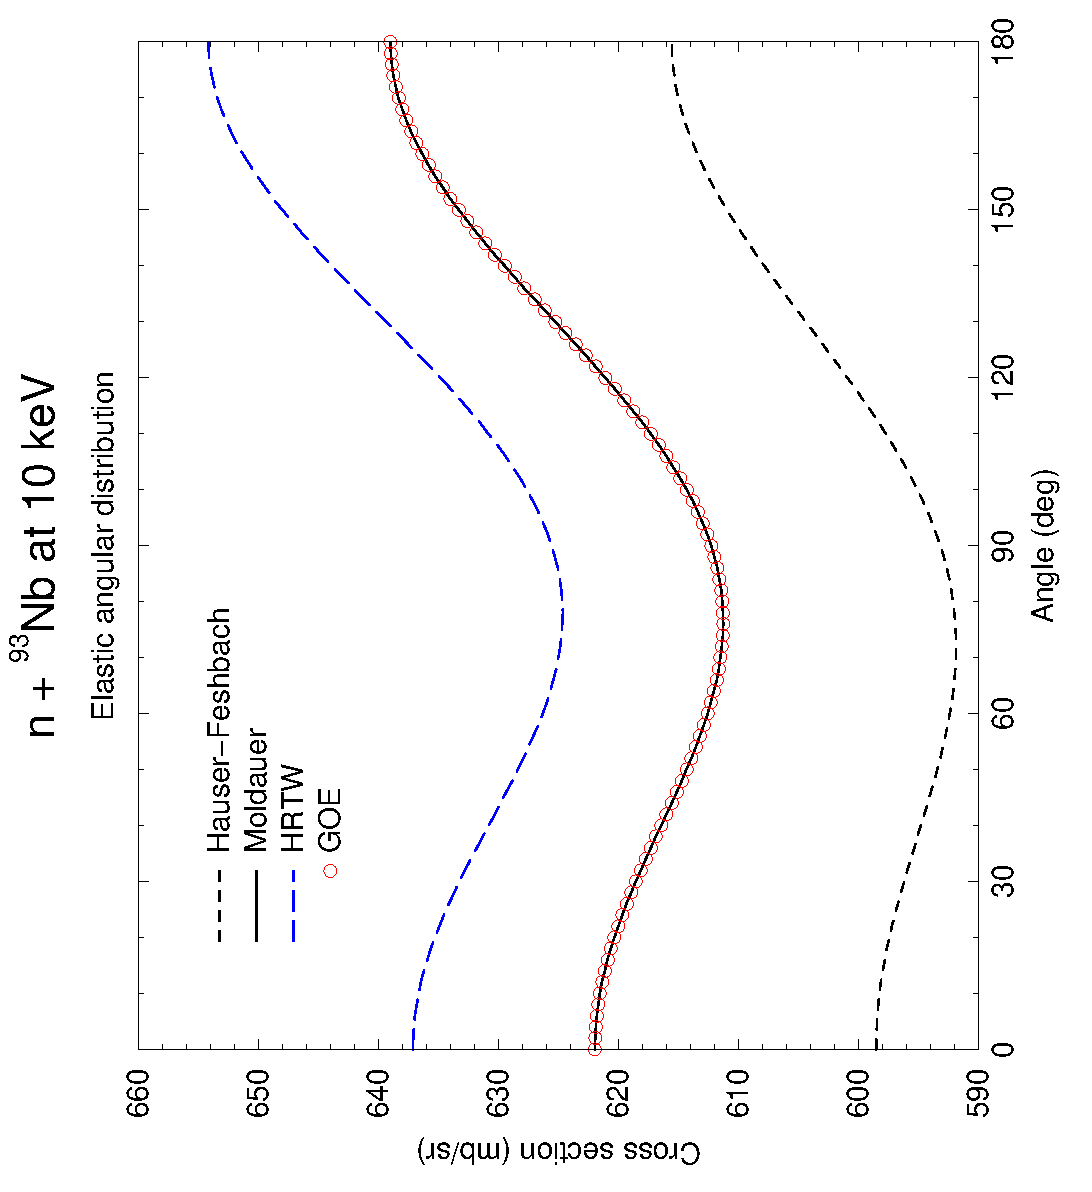
\includegraphics[scale=0.5,angle=270]{angwfc}
\caption{Total elastic angular distribution for 4 different compound nucleus
models for 10 keV neutrons incident on ${}^{93}$Nb.}
\label{angwfc}
\end{figure}
